\chapter{Introdução}


Dentre as inúmeras características que fazem um bom software, várias delas podem ser percebidas no código-fonte e algumas são exclusivas dele \cite{Meirelles2013}. Logo, decisões de desenvolvedores, que impactam fortemente sobre a qualidade do código-fonte, podem gerar trechos de código não coesos, que venham a se desfazer com o tempo e que aumentam exponencialmente a chance de manutenções corretivas onerosas \cite{Meirelles2013} \cite{beck2007implementation} \cite{beck1999}.



Portanto, avaliar continuamente a qualidade do código-fonte pode identificar antecipadamente trechos a serem melhorados, atingindo assim maiores graus de manutenibilidade, coesão, entendimento e legibilidade \cite{fowler1999refactoring}. Entre os vários métodos de análise da qualidade, está a análise estática de código-fonte, que se refere a uma análise automatizada das estruturas internas do código, em nível de linguagem de programação, sem realizar a execução do mesmo, com objetivo de obter métricas de código-fonte \cite{Terra2008} 
\cite{Emanuelsson2008} \cite{Wichmann95}  \cite{Nielson:1999} 
\cite{Sommerville10}. 

Durante anos, vários trabalhos foram publicados visando a definição formal de métodos de análise estática de código, como por exemplo, os trabalhos de \citeonline{Wichmann95}, 
\citeonline{Nielson:1999} e \citeonline{Emanuelsson2008}.
Contudo, as ferramentas que realizam este procedimento sobre o código-fonte 
apresentam alguns problemas, tais como:

\newlist{problems}{enumerate}{4}
\setlist[problems]{ label* = P\arabic* -}

\begin{problems}
    \item Ausência de resultados consolidados do produto, pois a maior 
	parte das métricas é extraída de elementos internos menores (Bibliotecas, 
	Pacotes, Classes, Métodos) do código-fonte.
    
	\item Ausência de mecanismos de tratamento, separação, recuperação, 
	organização e persistência de dados. 
	
	\item Ausência de associação entre resultados numéricos e forma de 
	interpretá-los: Ferramentas de análise estática frequentemente mostram 
	seus resultados como valores numéricos isolados para cada métrica 
	\cite{Meirelles2013}. 
	
	\item Em grande parte das ferramentas, a visualização dos resultados não é 
	agradável, isto é, é apresentado um conjunto de dados em uma janela 
	terminal contendo os valores das métricas.
	
    \end{problems}
	
Os problemas enunciados anteriormente trazem muitos prejuízos às organizações que 
utilizam processos de aferição de qualidade de código-fonte como um indicador do desenvolvimento de bons produtos de software, pois sem possibilidade de manter registros das métricas de código-fonte, torna-se inviável qualquer análise temporal da evolução da qualidade do produto de software. 

Dado este contexto, é crucial que dados relacionados às métricas sejam 
coletados e compartilhados entre projetos e pessoas em uma visão organizacional unificada, para que determinada organização ou time possa compreender o processo de medição e monitoramento de projetos de software e, 
consequentemente, se tornar mais hábil e eficiente em realizar atividades 
técnicas relacionadas ao processo de desenvolvimento de software 
\cite{Chulani2003}. 



Vários trabalhos têm mostrado que ambientes de \textit{Data Warehousing} 
(DWing) são boas soluções para atender à visão organizacional unificada de 
métricas de software proposta por \citeonline{Chulani2003}. Vide os trabalhos 
de \citeonline{Palza2003}, \citeonline{Ruiz2005}, \citeonline{Castellanos2005},
\citeonline{Becker2006}, \citeonline{Folleco2007}, \citeonline{Silveira2010}. 

Tendo os trabalhos, enunciados anteriormente, como o referencial teórico para ambientes de \textit{Data Warehousing}, adotou-se como questão de pesquisa deste trabalho: 


\newlist{questions}{enumerate}{3}
\setlist[questions]{ label* = Q\arabic* -}

\begin{questions}

	\item A visualização das métricas de código-fonte em ambientes de DWing confere maior visibilidade da qualidade geral do código-fonte de um determinado projeto?
	
\end{questions}


Com o intuito de verificar a questão de pesquisa, adotou-se como hipótese de pesquisa que \textbf{visualização e a extração 
de métricas de código-fonte em ambientes de DWing possibilitam as equipes maior poder de análise sobre a qualidade geral do código fonte quando comparada com as análises providas por ferramentas de análise estática de código-fonte isoladamente}. 


%-----------------------------------------------------------------------------%





%-----------------------------------------------------------------------------%

\section{Objetivos}

Esta seção apresenta o objetivo geral e os objetivos específicos deste Trabalho de Conclusão de Curso.

\subsection{Objetivo Geral}
Sob o prisma da questão de pesquisa, o objetivo geral deste trabalho é construir a visualização de métricas de código-fonte em um ambiente de \textit{Data Warehousing} (DWing) a fim de se validãr a hipótese de pesquisa.


%------------------------------------------------------------------------------%

\subsection{Objetivos Específicos}

Os objetivos específicos deste trabalho são:

\newlist{objectives}{enumerate}{3}
\setlist[objectives]{ label* = OE\arabic* -}

\begin{objectives}

	\item Construir o ambiente de DWing com ferramentas de software livre.

	\item Analisar a qualidade de um software livre a fim de instanciar a visualização das métricas de código-fonte em ambientes de DWing.
	
    \end{objectives}
	


%------------------------------------------------------------------------------%

\section {Metodologia de Pesquisa}

A metodologia de pesquisa deste trabalho foi construída em etapas. Para a primeira etapa, realizou-se pesquisa bibliográfica para a construção do referencial teórico. 

Na segunda etapa, realizou-se um estudo comparativo entre ferramentas livres para a construção do ambiente de \textit{Data Warehousing}. 

Após o levantamento das ferramentas, construiu-se o ambiente \textit{Data Warehousing}, em pequenos ciclos de produção. Para o acompanhamento das atividades de implementação, utilizou-se o Quadro \textit{Kanban}, que foi inventado pela Toyota com objetivo de controlar o fluxo da produção, mostrado na Figura \ref{kanban}.


\begin{figure}[h]
\centering
         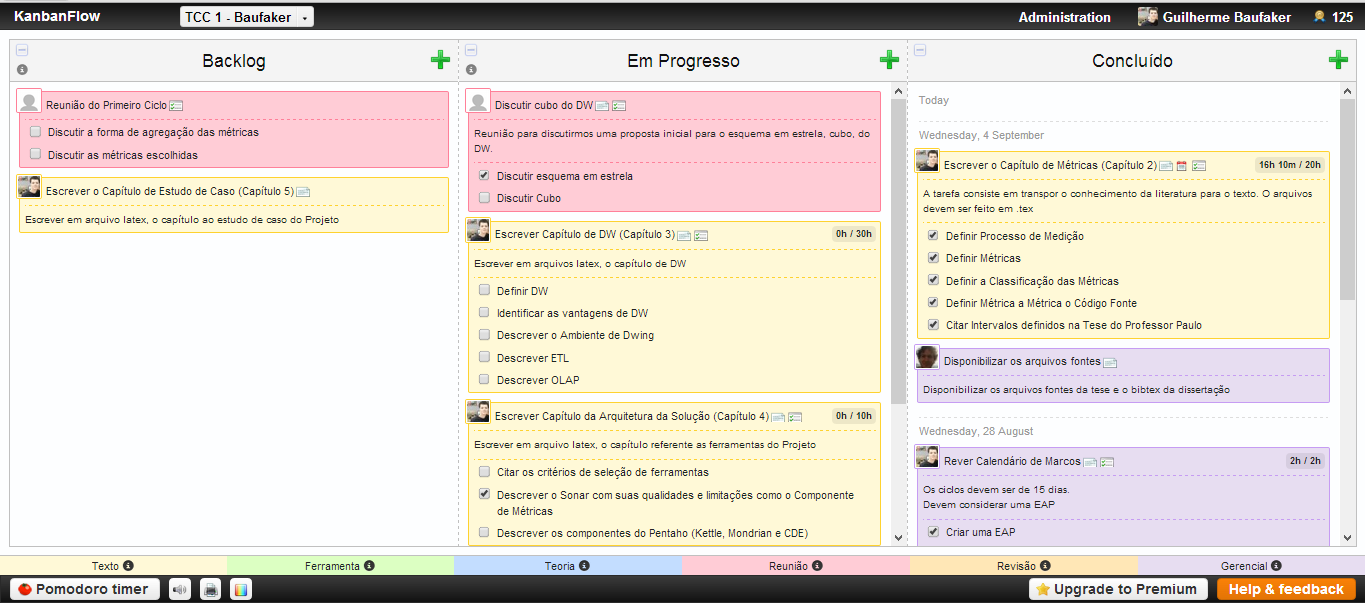
\includegraphics[keepaspectratio=true,scale=0.40]{figuras/kanban.eps}
         \caption{Quadro \textit{Kanban} do Trabalho de Conclusão de Curso}
         \label{kanban}
 \end{figure}

Após a construção do ambiente de \textit{Data Warehousing}, foi realizado um estudo de caso de coleta de métricas de código-fonte de um software livre com intuito de verificar a hipótese de pesquisa.


\section{Organização do Trabalho}

Para a primeira fase deste Trabalho de Conclusão de Curso, além desta 
introdução, o texto foi organizado em capítulos. O Capítulo 2 apresenta as 
métricas de software bem como o processo de medição, descrito pela ISO 15939, 
e as métricas de código-fonte. O Capítulo 3 
apresenta conceitualmente o ambiente de \textit{data warehousing} (DWing). O 
Capítulo 4 apresenta a implementação do ambiente de DWing construído neste 
trabalho. Por fim, o capítulo 5 apresenta as considerações finais com uso do 
ambiente de DWing na extração e visualização de métricas de código-fonte. 
